\documentclass[oneside]{book}

% 注意宏包顺序,有可能会报错
\usepackage{ctex}% 中文支持
\usepackage{geometry}% 用于页面设置
\usepackage[dvipsnames, svgnames, x11names]{xcolor}% 颜色支持
\usepackage{graphics}% 图形支持
\usepackage[
colorlinks=true,
linkcolor=Navy,
urlcolor=Navy,
citecolor=Navy,
anchorcolor=Navy
]{hyperref}% 设置超链接颜色
\usepackage{enumerate}% 枚举支持
\usepackage{tcolorbox}% 支持更好的文本框
\usepackage[english]{babel}% 载入美式英语断字模板
\usepackage{ulem}% 用于支持在字体上做下划线、波浪线等记号

% 设置为kindle 6英寸电子阅读器尺寸
\geometry{
	paperwidth = 9cm,
	paperheight = 12.2cm,
	margin = 0cm,
	left = 0.2cm,
	right = 0.2cm,
	top = 0.2cm,
	bottom = 0.5cm
}

\hyphenpenalty = 1000% 断字设置,值越大,断字越少。
\setmainfont{Ubuntu Mono}% 设置全局英文字体
\setlength{\parindent}{2em}% 缩进
\setlength{\parskip}{1ex} % 段间距

\let\svthefootnote\thefootnote

% 把目录区中英文的“Contents”改为中文的“目录”。
\addto\captionsenglish{
  \renewcommand{\contentsname}{目录}
}

% 把章节名称part、chapter换成中文
\usepackage{titlesec}% 可使用\usepackage[center]{titlesec}设置对齐方式
\titleformat{\part}{\centering\Huge\bfseries}{第\,\thepart\,部分}{0em}{\\}
\titleformat{\chapter}{\raggedright\Huge\bfseries}{第\,\thechapter\,章}{1em}{}
%\titleformat{\section}{\raggedright\Large\bfseries}{\,\thesection\,}{1em}{}

\includeonly{
  part1,
  part6,
}

% 定义指定字体名称与大小的文字输出命令
% 第1个参数:字体名称
% 第2个参数:字体大小
% 第3个参数:文本内容
\newcommand{\SetFont}[3]{
  \setCJKfamilyfont{font1}{#1} \CJKfamily{font1}\fontsize{#2}{#2}{\selectfont #3}
}

% 因为书中大量使用下划线,所以这里定义更为简便的命令来实现
\newcommand{\UL}[1][]{\underline{#1}}

% 定义不显示标号的脚注命令
\newcommand{\NoLabelFootnote}[1]{
  \begingroup
    \renewcommand\thefootnote{}\footnote{#1}
    \addtocounter{footnote}{-1}
  \endgroup
}


% ------------------ 开始 -------------------

\begin{document}

	% ------------------ 封面 -------------------
	\begin{titlepage}
		\pagecolor{black}
		\begin{center}
			\quad\\[20mm]
			\SetFont{FZKai-Z03S}{40}{\textcolor{Gold}{圣\quad 经}}
		\end{center}
	\end{titlepage}

	% ------------------ 前言 -------------------
	\frontmatter% 关闭章节序号,页码使用罗马数字
	\restoregeometry% 恢复导言区指定的页面布局。
	\nopagecolor% 清除封面创建时设置的背景色

	\pagecolor{WhiteSmoke}
	\begin{center}
		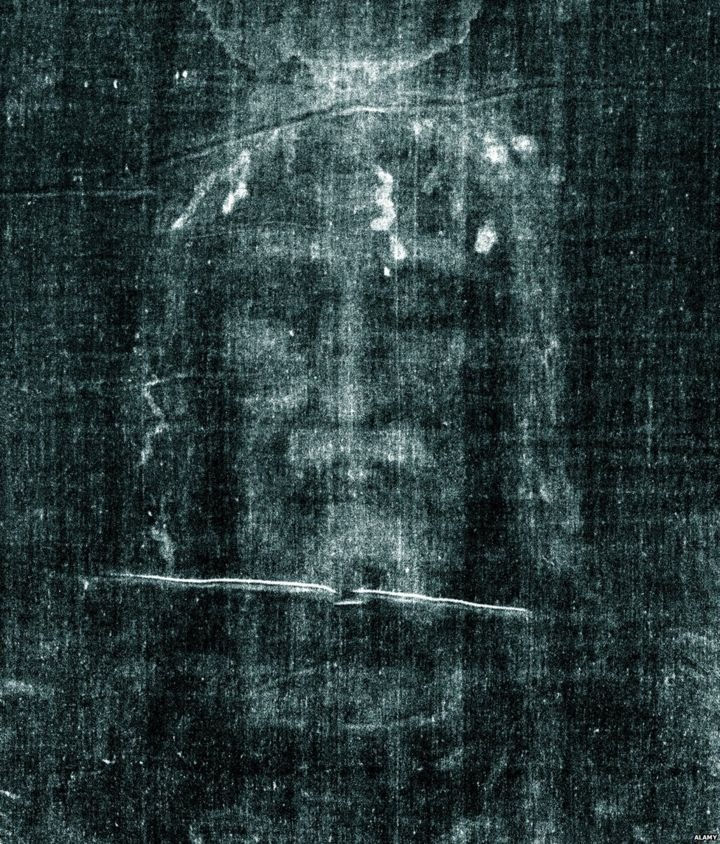
\includegraphics[width=8.5cm]{images/基督的面上闪耀着天主的光荣.png}

		\SetFont{zcoolqingkehuangyouti}{11}{“基督的面上闪耀着天主的光荣”}\normalsize\heiti(格后4:6)\songti
	\end{center}

	\newpage\normalsize
	\begin{center}
		\quad\\[10mm]
		承蒙联合圣经公会(United Bible Societies)

		为这一版本圣经的出版捐赠纸张,指定在中国

		大陆发行,谨此致谢!

		请为捐赠者祈祷。\\[10mm]

		With grateful thanks to United Bible

		Societies for the paper donated in

		the production of this Bible.

		This Bible is designated for distribution within mainland China only.

		Please pray for the donors.
	\end{center}

	\newpage
	\begin{center}
		\quad\\[15mm]
		\SetFont{FZKai-Z03S}{40}{圣\quad 经}
		\vfill
		\large\heiti 中国天主教主教团 准\normalfont\normalsize
	\end{center}

	\newpage
	\quad\\
	版权所有\copyright 思高圣经学会
	\vfill
	\begin{center}
		\Large 圣 经\normalsize

		——————————————

		发行者:中国天主教主教团

		承印者:南京爱德印刷有限公司

		准印证号:Z(2018)00000522
	\end{center}

	\newpage
	\quad\\\\
	\centerline{\heiti\large 前\qquad 言}\songti\normalsize

	\quad

	为了满足广大神长教友的需求,经中国天主教主教团批准,现将旧、新约合订本《圣经》印制发行。并再次感谢香港思高圣经学会的帮助。

	《圣经》是一部在天主圣神默示下写成的圣书,天主的话是圣教会及众信友的生命泉源,是不可缺少的精神食粮,愿神长教友在圣教会的训导下,虔诚地、认真地阅读、默想《圣经》,聆听基督的圣训,在爱主爱人的道路上不断圣化自己,为主作证。\\\\
	\mbox{\quad}\hfill 中国天主教主教团\mbox{\qquad\quad}\\
	\mbox{\quad}\hfill 2009年2月\mbox{\qquad\qquad}

	\newpage
	\quad\\\\
	\centerline{\heiti\large 序}\songti\normalsize

	\quad

	中文《新旧约》合订本,几经艰辛,终于出版面世了。现在谨以孝爱的心肠,与兴奋的心情,将此书献给我国的天主教会。我们由衷地感谢万善万美之源在天之父,虔恭地恳求他,降福我们的每一位神形恩友。我们明知,如果没有他们精神方面的支持与物质方面的援助,这部\UL[中]译圣经合订本、很难于今日完成。我们更恳求天父,以圣神的恩泽,充溢每位读者的心灵,为光荣他,和他的圣子,我们的救主\UL[耶稣]\UL[基督]。最后,我们以至诚的心,深望每位读者,效法天主之母,童贞圣母\UL[玛利亚],常将天主子\UL[耶稣]\UL[基督]的奥迹,默存于心,反复思念(\uwave{路}2:19、51)。

	我们坦诚地说过应说的话以后,兹将有关出版这部合订本的原则与方法,向诸位读者报告如下:

	本学会同仁,对本学会以前的译文,作了一次彻底的修订;特别对于《旧约》部分,觉得有重新翻译的必要。这次的修订,一如以往翻译一样,仍旧依据原文,即\UL[希伯来]、\UL[阿剌美]和\UL[希腊]文,间或有时依据古译本,将艰涩的经文稍加修改,很少采用近代学者的臆测。为了促进合一运动,我们在《新约》的修订工作上,曾参考了最近基督教五个圣经公会联合印行的《圣经》希腊版本。这版本是1966年由\UL[艾朗德](Aland)\UL[白赖克](Black)\UL[墨则格](Metzger)\UL[魏革伦](Wikgren)四位极负盛名的学者所细心校勘的。不过,在选择异文方面,有时我们未能尽表赞同或采纳。然而,众所周知,在校勘方面,要想使所有学者的意见,完全趋于一致,几乎是不可能的事;同时,艰深疑难的问题,也实在可说是无法解决;但为了遵守有助于合一运动的措施,我们仍尊重而参考了他们的意见。

	在翻译《多俾亚传》和《友弟德传》时,我们采用了《西乃抄卷》,因而与\UL[拉丁]通行本和其他控译本,略有出入,因为这些译本,大半是根据《亚历山大抄卷》或《梵蒂冈抄卷》而译成的。

	《德训篇》一书,我们虽译自\UL[希腊]文,但同时也参考了最近在古\UL[开罗]的旧书库中,以及在\UL[死海]近旁的\UL[古木兰],和1965年在\UL[玛撒达]所发现的本书\UL[希伯来]文残卷。为了更进一步了解本书\UL[希腊]译者的愿意,我们自始至终,将\UL[希腊]本,与古\UL[拉丁]译本和《叙利亚培西托》译本,加以比较和对正。至于\UL[拉丁]通行本所特有的辞句,我们仍旧全部保留,以小字体排印;我们如此作,是因为这些经文往往与\UL[希伯来]文残卷和\UL[叙利亚]译本相吻合;尤其因为在\UL[拉丁]教会内,许多世纪以来,在礼仪上采用了这些经文。至于本书的音节,全依\UL[拉丁]通行本排列。

	至论《圣咏集》的翻译,虽也译自\UL[希伯来]原文,但我们却作了一个新的尝试,就是放弃了过去无韵文的翻译,而试作有韵文的翻译。采取这种翻译的理由,是为了在礼仪上便于诵读。

	为了切合实际,我们尽量缩短了每卷的引言和注释。对于那些欲求圣经高深知识的读者,我们仍建议,请他们参考本学会以前出版的《圣经》各卷注释。对于那些工作繁重与事务缠身,而没有充分时间的读者,我们认为本书的引言、注释以及各种附录和图表,已够他们了解《圣经》的主旨。如果读者能进一步,如圣教会所期望的,以祈祷和默祷的方式阅读本书,则更受益匪浅。

	现在再向读者特别介绍本书后面的三种附录,这类附录在\UL[中]文《圣经》方面尚属少见。

	一、“历代大司祭一览表”:读者可从这表内,正确地明晰一切有关宗教事务的事实,发生于何时何代,发生在哪一位大司祭的任期中。

	二、“圣经与世界大事年表”:在这表内,我们以编年体,将选民的历史,以及与选民有关的其他民族的历史,和我们\UL[中华]民族的历史,加以比较,列表阐明。我们认为这一附录,可使我国同胞,更方便而有效地传诵救恩史。

	三、“圣经教义索引”:这是为了符合\UL[梵蒂冈]第二届大公会议的期望,而特别编制的,目的是使信友迅速而无误地,直接从圣经中吸取天主启示的各端要理,走上愈显天父的光荣,生活于基督内的康庄大道。我们希望藉此索引,得到抛砖引玉的效果,就是说,希望每位读者藉此索引,能将救恩史的大纲,加以质的扩充和量的增补。

	至于地理图表,以及其他有关圣经的插图,都是参照专家和学者们最新的探讨与研究的心得,而予以重新编制的。本书的题字“圣经”、“旧约”、“新约”、六字,是临自《大秦景教流行中国碑》。

	最后,我们愿用一首庄严而又古雅的赞颂辞,向我全国教胞表达我们的心愿,并结束这篇序文:愿光荣藉着天主圣子,在天主圣神内,并在圣教会内,永远归于天主圣父!\\

	\mbox{\quad}\hfill 思高圣经学会谨识于香港\\
	\mbox{\quad}\hfill 1968年8月15日\mbox{\quad}\\
	\mbox{\quad}\hfill 圣母升天瞻礼\mbox{\qquad}

	\newpage
	\quad

	\centerline{\large\textbf{凡\qquad 例}}\normalsize

	(一)本书中人名地名,除教会与普通常用者外,大抵依原文音译。

	(二)本书引言、注释引用的经文,概以本书译文为根据。

	(三)凡后人所加,或由他处窜入的经文,概置于方括弧内。

	(四)*号表示原文无,只见于\UL[拉丁]通行本。

	(五)《新约》经文引用《旧约》经文,概括以‘ ’引号。

	(六)引言、注释内,如引用原书经文,则不标书名,只标章节。

	(七)引言、注释内,注明出处时,章数、节数按如下表示:如\uwave{依}3:6,即《依撒意亚》第3章第6节;如一书没有章数,则节数按以下标出:如\uwave{北}8,即《亚北底亚》8节。

	% ------------------ 目录 -------------------
	\tableofcontents% 生成目录

	% ------------------ 正文 -------------------
	\mainmatter%

	\part{旧约}


\chapter*{新旧约全书总论}
《新旧约全书》是数十卷经书的总集。这些经书的特点,在于它们的写成有超乎自然之处,因为这些经书都是在天主对神默感下写成。赐予天主的子民——教会——的礼品。

圣教会自古以来,一致主张这部总集包括《旧约》46卷,《新约》27卷,共计73卷。但大多数的\UL[基督教]派,由于只相信以\UL[希伯来]文写成的书才为圣经,因此现今只有\UL[希腊]原文的《巴路克》、《多俾亚传》、《友弟德传》、《玛加伯》上下、《智慧篇》和《德训篇》7卷,未著录在他们的圣经书目内。而天主教会自古即以\UL[希腊]文七十贤士本为圣经,因而对上述7卷也一律认为是圣经。

这些经书称为“约“,因为其中心思想,是天主与人类所立的盟约。天主与\UL[以色列]民族在\UL[西乃]山上所立的盟约,称为“旧约“;\UL[耶稣]以自己的圣血和圣死为全人类所立的永远盟约,称为“新约“。这些经书又称为“圣经“,是为表示这些书所具有的独特地位和神圣权威。书中所记述的一切,是吾人信仰及道德的大经,又为吾人立身经世的大道。

《旧约》经书的原文,除几卷和几小段外,大都以\UL[希伯来]文写成。后来侨居\UL[北非]受了\UL[希腊]文件影响的\UL[犹太]人,因多不谙\UL[希伯来]文,\UL[犹太]人遂在公元前三至二世纪,将《旧约》各书译为\UL[希腊]文,即今所称的“七十贤士译本“。以后\UL[希腊]文\footnote[0]{原书为“语文“}也成了\UL[罗马]帝国的通用语言,宗徒们在各宣讲福音,为了方便起见,即时常利用这部\UL[希腊]文圣经。为此这部\UL[希腊]文圣经(包括46卷)自初即为教会所尊重,并具有极大的权威。

《新约》各书,全部是以\UL[希腊]文写成,只有《玛窦福音》,原文虽为\UL[阿辣美]文,但很早即已失传;今所留传的,只有\UL[希腊]文本。

《旧约全书》的写成,凡经一千余年(约由公元前1300至100年),而逐渐汇为一集。《新约全书》是公元初世纪宗徒时代的作品。

《新旧约全书》,通常分为三大类:即历史书、先知书和智慧书(或训诲书),这是很广泛的分类。至于作者,《旧约》大多出于先知及其他贤哲的手笔,《新约》是宗徒和宗徒弟子的写作。但因全部圣经都是“因天主的默感写成的“(\uwave[弟]后3:16),经内的话是“由天主所派遣的圣人,在圣神推动之下说出来的“(\uwave[伯]后),为此我们不得不承认圣经的首要作者是天主。所谓“默感“,即是说:圣经的作者与编者(人),在天主的灵性感动之下,写下天主愿向他的子民(旧约与新约的教会)所要说的话,记下天主要他们记述的史事。有时天主也曾向他们透露某些重要的事迹,或直接向他们说话;这样,作者不仅获得了“默感“,同时也获得了“启示“。既然天主是圣经的首要作者,那么圣经上所记载的即是天主的话,即是天主的“圣言“。既然是天主的话,那么圣经上所载的一切,句句都是“真实无误“。就是说:圣经作者在天主默感下所愿表示出来的意义,是不会错误的。但为了解作者所要表达的本意,必须先注意经书中每部书的文体和体裁:是散文或是诗体?是历史或是传奇?是寓言或是训诲?因为每种文体有其独特的意义。同时还应注意作者或编者的时代背景,因为时代不同论事的观点也各有异。比如古代民族,尤其\UL[以色列]人对历史的观点,和今日的史学家的观点,有绝大的不同。尤其圣经的作者或编者,是本着宗教观点来编述历史的过程。他们看历史时,常着眼于天主为历史的推动者和支配者;人民的盛衰兴亡,常系之于他们是否遵守天主的法律。

另一个极重要的问题,是圣经与科学。圣经的作者决无意又教授自然科学(如宇宙学、天文学、生物学、人类学等)为写作的目的。圣经作者的目的,是在于启迪人类“获得拯救的智慧”(\uwave{弟}后3:15);为此他们无意研究自然界的进化和人体的构造,其用意识在说明自然界和人类与天主的关系,教导世人,天地万物都来自天主,一切都因天主的照顾而生存,最后又归于天主。

还就当注意的是:为适当地研究圣经和解释经意,人人必须先有信仰,并甘心接受圣教会的指导,因为天主把圣经委托给教会保管,因此只有教会才有解释圣经的特权。

圣经中所记载的都是些最重要的真理。教父多称圣经为天主给流徙的世人寄来的家书或天书。在这部天书内,天主先将自己启示给世人并告知世人,天地万物的来历和目的,告诉我们天主原先怎样给人类备下了幸福,现今的痛苦、患难和死亡又怎样来的;天主在漫长的历史过程中,怎样逐步实现了他救赎人类的大计划。《旧约》》所载,即是天主为\UL[以色列]民族所行的大事,所定的法律,所发的劝言和警告。这一切都是他为完成救赎人类工程的准备,甚至\UL[以]民的被选,也是为准备万民获得救恩。《新约》则是全人类得救的大喜讯,记载着人类唯一的救主\UL[耶稣]\UL[基督]救赎人类的大事;因为\UL[耶稣]是天主第二位圣子,只有他才能把天主性的真理启示给人类。他降生成人,藉着自己的人性,完成了天主慈爱的计划,使人与天主重归于好,且提高了人类的地位,使人分享天主性的永福。

由此看来,\UL[耶稣]\UL[基督]实为《旧新》二约的中心,是“法律”(旧约)的终向(\uwave[罗]10:4),是“新约的中保”(\uwave[希]8:6)。《旧新》二约各经卷的最后目的,就是叫人准备期待“我们伟大的天主及救主耶稣基督的光荣显现”(\uwave[铎]2:13)。

圣经为人类得救既有如此重要的关系,因此圣经对圣教会,对于一切基督信徒,对全人类,的确是举世无双的无价宝书。圣\UL[保禄]论《旧约》说:“凡所写的,都是为教训我们写的”(\uwave{罗}15:4),“为教训,为督责,为矫正,为教导人学正义,都是有益的”(\uwave{弟}后3:16)。这些话对《新约》来说,更为恰当;而且可说,如果没有圣经,我们无论对天主,或是对人,不会有一个正确的认识,因为只凭理性的自然神学是不够的,决不能打动人心,惟有研读圣经才能触及我们灵魂的深处,使我们听得见“生活天主”的话,领略天主威爱兼有的声音,洞见他全能的伟大化工,明白他怎样生养保存万物,怎样怎样以他至高无上的主权宰治一切,裁判一切;又怎样以他交慈父心肠,导引迷途的荡子,回归父家。无怪乎教宗\UL[良]十三称圣经为“神学的灵魂”。

诚然,一个怀有信德的教友,在恭读默思圣经时,应觉得是与天主会晤,是在静听天主的劝导,是在听他在天之父的慈音。当他心有所得,情有所动时,自然就向天主说话,这即是祈祷。无怪乎圣教会自古即以圣经为赞美、祈祷、默想最好的宝书。信友如能日日如此读经,与天主互诉衷曲,在日常的生活上或工作上,性能时时对越天主,承行他的圣意,臻于圣化一切的至境。为此教会不断劝勉信友多读圣经,尤其这次大公会议,对圣经研究与圣经诵读特予强调。愿我信友善体慈母教会的劝告,勉力天天去阅读这部天赐宝书。


\chapter*{梅瑟五书引论}
《旧约全书》前五卷,通称“梅瑟五书”,或简称“五书”。因为在这五卷书内,包含着《旧约》中最重要的一部分,即\UL[梅瑟]给\UL[以色列]人所宣布的法律,为此圣经上多次称《五书》为“法律”。\UL[希伯来]人称之为“托辣”。

《梅瑟五书》虽然在纪元前已有如此的分划:即《创世纪》、《出谷纪》、《肋未纪》、《户籍纪》、《申命纪》,但自古以来这五卷书常视为一部,且是一部世界文学上的杰作。

如果说全部圣经的主题是阐述人类的救赎史,那么“五书”即是记述这救赎史的开端。作者从天地和人类的创造开始,说到人类因违背天主的命令,而失掉原有的幸福,再扼要地叙述各民族的太古史,继而只着重于\UL[以色列]民族的起源,及其成为天主选民的历史。这历史的中心即在于天主与选民在\UL[西乃]山上所结的盟约。天主很早即对\UL[以色列]人的先祖再三地许诺,要以特殊照顾和非凡的奇事,准备\UL[以]已的心灵,使他们对天主养成坚定不移的信仰,以后好藉\UL[梅瑟]选立他们为自己的国民,颁下当遵行的法律,在世上建立起神权政体的神国。以后又在旷野四十年之久,以种种试探考验了他们的忠诚和信心;最后引他们到了\UL[约但]河东岸,在那里又藉\UL[梅瑟]劝告他们,重述以前教导过他们的一切,准备他们进占已预许给他们祖先的福地。所以从历史方面来看,“五书”有其统一的目标,实是一部上下一贯的著述。

按古来一致的传授,“五书”的作者是\UL[梅瑟]。称他为作者,并不是说全书每字每句都出于他一人的手笔,而是说他曾搜集了不少当时所能找得到的史料、文献和法律。且在他死后,有许多历史或法律部分是后人增补的,因为“五书”原是\UL[以色列]人宗教、政治、社会生活的法典,所以常有随时增添一些解释的必要,为使\UL[梅瑟]法律能随历史的演变,而适应时代的环境。

从以上所述,可知“五书”为\UL[以色列]人具有多么重要的关系。如果我们对“五书”没有认识,便不能明了\UL[以色列]子已的历史,因为他们生活在一个神权政体的制度之下,他们的存亡盛衰,全系于他们是否忠实履行天主藉\UL[梅瑟]所颁布的法律。在《旧约》其他经书内,常不断指出法律的这种重要关系,并依法律为原则,来批判一切历史的得失。但这法律的最终目的,诚如圣\UL[保禄]所说:“法律的终向本来是基督”(\uwave{罗}10:4)。为此,法律为\UL[以色列]人,好像是“归于基督的启蒙师”(\uwave{迦}3:24)。换句话说,法律应领导\UL[以色列]人,认识并信仰将要来临的默西亚。当默西亚\UL[耶稣]\UL[基督]一降生,法律的使命就算完结,\UL[耶稣]所宣讲的“爱的诫命”,满全了整个法律(\uwave{罗}13:10)。虽然如此,“五书”为《新约》的教会,仍未失其重要性,因为本书含有永生天主的启示,以及教会信仰的基础。


\chapter*{创世纪引言}
“梅瑟五书”每部的名称,\UL[犹太]人皆以每书的首句首字为名。自\UL[希腊]七十贤士译经以来,皆以每书的内容大意命名。“梅瑟五书”的第一部名为《创世纪》,因为本书并不是以科学的论点和近代史学家的方法来记述,而是本着宗教的观点来说明救赎史的开端。在这救赎史中,依照天主的计划,\UL[以色列]民族在万民中占着重要的角色,因此作者也只着重于这个民族的历史。

本书的前编(1-11章),是救世史的前导,说明天主是整个天地万物的创造者,和全人类历史的领导者;并指出\UL[以色列]人与其他民族的关系。原父母虽然背命,惹下了滔天大祸,后继的人们也多半背弃了天主,如洪水和\UL[巴贝耳]塔时代的人,但因为人是按天主的肖像造成的,天主决不愿将全人类完全抛弃,所以在后编内(12-50章),作者便记述天主怎样拣选了一位信仰坚定,服从听命的人——\UL[亚巴郎],怎样向他起誓,立他为一个新民族的始祖,即将来要成为天主选民的民族的始祖,许下因他和他的后裔,天下万民将要获得祝福(22:18),由他的后裔中要生出一位“应得权杖,万民都要归顺他”(49:10),他要使“救恩达于地极”的后裔(\uwave{依}49:6)。在记述\UL[亚巴郎]、\UL[依撒格]、\UL[雅各伯]和\UL[若瑟]的事迹中,作者一再证明天主怎样特殊地照顾了他们,以准备救赎人类的道路。


\chapter{创世纪}


\section{前编  太古史(1-11)}


\subsection{第一章 天地万物的创造}
\renewcommand{\thefootnote}{\alph{footnote}}

$^{1}$在起初天主创建了天地。$^{2}$大地还是混沌空虚,深渊上还是团黑暗,天主的神在水面上运行。\footnote{1 “在起初……”一语,暗示创造万物之时,除天主外,一无所有。“天地”二字此处有宇宙万物之意。作者用诗人的相像力描写天主好似一个工程师,在六天以内创造了万物,到第七天休息。首先所创造的是混沌的无生之物,后将这混沌之物分成天、地、海三大部分,然后以日月、星辰、草木、飞禽、走兽等来点缀天地海洋。最后天主照自己的肖像造了人。作者从创造混沌之物说起,到创造人,表示人是万物之灵,应效法造物主工作和守安息日。此开宗明义第一章是远古时代的文学杰作,是一篇宗教的重要文告,并不是自然科学的论著。按古代各民族对天地开辟,人类诞生的传说,没有可与《创世纪》第一章相比拟的。“天主的神”指施生命之神力,但若通观新旧二约的全部启示,此处也指赐生命的“天主圣神”。}$^{3}$天主说:“有光!”就有了光。$^{4}$天主见光好,就将光与黑暗分开。$^{5}$天主称光为“昼”,称黑暗为“夜”。过了晚上,过了早晨,这是第一天。

$^{6}$天主说:“在水与水之间要有穹苍,将水分开!”事就这样成了。$^{7}$天主造了穹苍,分开了穹苍以下的水和穹苍以上的水。$^{8}$天主称穹苍为“天”,天主看了认为好。过了晚上,过了早晨,这是第二天。

$^{9}$天主说:“天下的水应聚在一处,使旱地出现!”事就这样成了。$^{10}$天主称旱地为“陆地”,称水汇合处为“海洋”。天主看了认为好。$^{11}$天主说:“在陆地上,土地要生出青草、结种子的蔬菜和结果子的果树,各按照在它内的种子的种类!”事就这样成了。$^{12}$土地就生出了青草,结种子的蔬菜,各按其类,和结果子的树木,各按照在它内的种子的种类。天主看了认为好。$^{13}$过了晚上,过了早晨,这是第三天。

$^{14}$天主说:“在天空中要有光体,以分别昼夜,作为规定时节和年月日的记号。$^{15}$要在天空中放光,照耀大地!”事就这样成了。$^{16}$天主于是造了两个大光体:较大的控制白天,较小的控制黑夜,并造了星宿。$^{17}$天主将星宿摆列在天空,照耀大地,$^{18}$控制昼夜,分别明与暗。天主看了认为好。$^{19}$过了晚上,过了早晨,这是第四天。

$^{20}$天主说:“水中要繁生蠕动的生物,地面上、天空中要有鸟飞翔!”事就这样成了。$^{21}$天主于是造了大鱼和所有在水中孳生的蠕动生物,各按其类,以及各种飞鸟,各按其类。天主看了认为好。$^{22}$遂祝福它们说:“你们要孳生繁殖,充满海洋;飞鸟也要在地上繁殖!”$^{23}$过了晚上,过了早晨,这是第五天。

$^{24}$天主说:“地上要生出生物,各按其类;走兽、爬虫和地上的各种生物,各按其类!”事就这样成了。$^{25}$天主于是造了地上的生物,各按其类;各种走兽,各按其类;以及地上所有的爬虫,各按其类。天主看了认为好。$^{26}$天主说:“让我们照我们的肖像,按我们的模样造人,叫他管理海中的鱼、天空的飞鸟、牲畜、各种野兽、在地上爬行的各种爬虫。”$^{27}$天主于是照自己的肖像造了人,就是照天主的肖像造了人:造了一男一女。$^{28}$天主祝福他们说:“你们你们要生育繁殖,充满大地,治理大地,管理海中的鱼、天空的飞鸟、各种在地上爬行的生物!”\footnote{1 “人”按原文有红土或黄土的意思,是说人是属于土的造物。“我们”(26节)按古\UL[犹太]经师的解释,是指天主和天使,好似天主同天使商量;但有些学者主张为“威严复数”或“议决复数”。教父和神学家多以为此复数暗示天主圣三的奥理。此说若照启示的演进说是对的。人相似天主是按灵魂说的,相似天主有理智、意志和记忆。论人的肉身,当天主造\UL[亚当]时,已预见作\UL[亚当]第二的\UL[基督](\uwave{罗}5:14)。“造了一男一女”,指婚姻一夫一妻制和不可分离性(\uwave{玛}19:1-6;\uwave{拉}2:15、16)。天主祝福原祖生育繁殖的话,说明婚姻的首要目的是生养教育子女(8:17;\uwave{咏}127:3、4)。}$^{29}$天主又说:“看,全地面上结种子的各种蔬菜,在果内含有种子的各种果树,我都给你们作食物;$^{30}$至于地上的各种野兽,天空中的各种飞鸟,在地上爬行有生魂的各种动物,我把一切青草给它们作食物。”事就这样成了。$^{31}$天主看了他造的一切,认为样样都很好。过了晚上,过了早晨,这是第六天。\footnote{1 天主造了原祖,也赐给了他们和他们传生的人类食物,并将普世交给他们统治。所造的万物样样都好,是说万物都合天主的旨意,都为他所喜爱。参阅\uwave{咏}19:1-6,104,145,148,150。}


\subsection{第二章 安息日}
$^{1}$这样,天地和天地间的一切点缀都完成了。$^{2}$到第七天天主造物的工程已完成,就在第七天休息,停止了所作的一切工程。$^{3}$天主祝福了第七天,定为圣日,因为这一天,天主停止了他所行的一切创造工作。\footnote[1]{2 1-3节属前章,劝人守安息日为圣日。守安息日的原因与目的,见\uwave{出}23:12;\uwave{申}5:12-15。}


\subsubsection{人与乐园}
$^{4}$这是创造天地的来历:在上主天主创造天地时,$^{5}$地上还没有灌木,田间也没有生出蔬菜,因为上主天主还没有使雨降在地上,也没有人耕种土地,$^{6}$有从地下涌出的水浸润所有地面。$^{7}$上主天主用地上的灰土形成了人,在他鼻孔内吹了一口生气,人就成了一个有灵的生物。$^{8}$上主天主在\UL[伊甸]东部种植了一个乐园,就将他形成的人安置在里面。$^{9}$上主天主使地面生出各种好看好吃的果树,生命树和知善恶树在乐园中央。\footnote{2 2:4-3:24为创造天地万物的另一记载。原来在这记载中只用了上主(雅威)的名词,但将这个记载与上章的记载编在一起时,补入了“天主”的名词。这记载的中心为人:天主对人,人对天主的态度。关于人的来历和本性,作者用简略的话,教训人一端论宗教和文化的最高深的道理:人肉身的形成,好像其他的动物,是由尘土造成的,但对于灵魂却有极大的区别,它是直接由天主所造。\UL[伊甸]乐园位于何处,人不得而知。乐园是天主考验人的地方。“生命树”所象征的是天主愿意赐给人的“不死”之恩。“知善恶的树”,是试探人的工具。“知善恶”的意思,大概是说:人一犯天主的禁令,就知道所失去的超性恩宠——真善,是多么完善,所犯的罪恶——真恶,是如何凶恶。}$^{10}$有一条河由\UL[伊甸]流出灌溉乐园,由那里分为四支:$^{11}$第一支名叫\UL[丕雄],环流产金的\UL[哈威拉]全境;$^{12}$那地方的金子很好,那里还产珍珠和玛瑙;$^{13}$第二支河名叫\UL[基红],环流\UL[雇士]全境;$^{14}$第三支河名叫\UL[底格里斯],流入\UL[亚述]东部;第四支河即\UL[幼发拉的]。$^{15}$上主天主将人安置在\UL[伊甸]的乐园内,叫他耕种,看守乐园。\footnote{2 说明人犯罪之前,天主已叫人应该工作。}$^{16}$上主天主给人下令说:“乐园中各树上的果子,你都可吃,$^{17}$只有知善恶树上的果子你不可吃,因为那一天你吃了,必定要死。”


\subsubsection{造女人立婚姻}
$^{18}$上主天主说:“人单独不好,我要给他造个与他相称的助手。“$^{19}$上主天主用尘土造了各种野兽和天空中的各种飞鸟,都引到人面前,看他怎样起名;凡人给生物起的名字,就成了那生物的名字。$^{20}$人遂给各种畜牲、天空中的各种飞鸟和各种野兽起了名字;但他没有找着一个与自己相称的助手。$^{21}$上主天主遂使人熟睡,当他睡着了,就取出了他的一根肋骨,再用肉补满原处。$^{22}$然后上主天主用那由人取来的肋骨,形成了一个女人,引她到人前,$^{23}$人遂说:“这才真是我的骨中之骨,肉中之肉,她应称为“女人“,因为是由男人取出的。“$^{24}$为此人应离开自己的父母,依附自己的妻子,二人成为一体。$^{25}$当时,男女二人都赤身露体,并不害羞。\footnote{2 本段的要义有二:一、人给动物命名,是表示人受有统治一切造物的权柄;二、从\UL[亚当]的肉身形成了第一个女人,是指女人同他有一样的人性,像\UL[亚当]一样是照天主的肖像受造的。夫妇结为一体,表示婚姻的结合是天主制定的,人不能拆散(\uwave{玛}19:5、6)。赤身不害羞,是说原祖未犯罪前纯洁无罪的状态,还未体验到罪过的恶果。}


\subsection{原祖违命}
$^{1}$在上主天主所造的一切野兽中,蛇是最狡猾的。蛇对女人说:“天主真说了,你们不可吃乐园中任何树上的果子吗?“$^{2}$女人对蛇说:“乐园中树上的果子,我们都可吃;$^{3}$只有乐园中央那棵树上的果子,天主说过,你们不可以吃,也不可摸,免得死亡。“$^{4}$蛇对女人说:“你们决不会死!$^{5}$因为天主知道,你们那天吃了这果子,你们的眼就会开了,将如同天主一样知道善恶。“$^{6}$女人看棵果树实在好吃好看,令人羡慕,且能增加智慧,遂摘下一个果子吃了,又给了她的男人一个,他也吃了。$^{7}$于是二人的眼立即开了,发觉自己赤身露体,遂用无花果树叶,编了个裙子围身。$^{8}$当\UL[亚当]和他的妻子听见了上主天主趁晚凉在乐园中散步的声音,就躲藏在乐园的树林中,怕见上主天主的面。\footnote{3 本章记的蛇就是魔鬼。他藉蛇形诱惑了\UL[厄娃](\uwave{智}2:23、24;\uwave{若}8:44;\uwave{默}12:9,20:2)。原祖所犯是骄傲背命的罪。“发觉自己赤身“,是指失去天主的宠爱和原始的纯洁。}$^{9}$上主天主呼唤\UL[亚当]对他说:“你在哪里?“$^{10}$他答说:“我在乐园中听到了你的声音,就害怕起来,因为我赤身露体,遂躲藏了。“$^{11}$天主说:“谁告诉了你,赤身露体?莫非你吃了我禁止你吃的果子?“$^{12}$\UL[亚当]说:“是你给我作伴的那个女人给了我那树上的果子,我才吃了。“$^{13}$上主天主遂对女人说:“你为什么作了这事?“女人答说:“是蛇哄骗了我,我才吃了。“\footnote{3 天主询问时,没有询问魔鬼,只询问了\UL[亚当]\UL[厄娃];但惩罚时却按罪过的原因和轻重;先是魔鬼,后是\UL[厄娃],最后是\UL[亚当](\uwave{弟}前2:13-15)。}


\subsubsection{处罚与预许}
$^{14}$上主天主对蛇说:“因你做了这事,你在一切畜牲和野兽中,是可咒骂的;你要用肚子爬行,毕生日日吃土。$^{15}$我要把仇恨放在你和女人,你的后裔和她的后裔之间,她的后裔要踏碎你的头颅,你要伤害他的脚跟。”$^{16}$后对女人说:“我要增加你怀孕的苦楚,在痛苦中生子;你要依恋你的丈夫,也要受他的管辖。”$^{17}$后对\UL[亚当]说:“因为你听了你妻子的话,吃了我禁止你吃的果子,为了你的缘故,地成了可咒骂的;你一生日日劳苦才能得到吃食。$^{18}$地要给你生出荆棘和蒺藜,你要吃田间的蔬菜;$^{19}$你必须汗流满面,才有饭吃,直到你归于土中,因为你是由土来的;你既是灰土,你还要归于灰土。”\footnote{3 天主的传递既超过了他的公义,故此他在义怒中给人类预许了人终要得胜魔鬼的诺言;因这许诺,3:15称为“原始福音”。大义是:踏碎蛇头是得胜魔鬼的象征;“女人的后裔”虽然也指犯罪败坏的人类,但在此特别指拯救人类的新元首\UL[基督](\uwave{哥}1:15-18),只有他打败了魔鬼;故此圣\UL[保禄]称他为“新\UL[亚当]”(\uwave{罗}5:12-15)。魔鬼同\UL[厄娃]的对白,与天使同\UL[玛利亚]的对白恰恰相反:一是诱惑的对白,一是商讨救赎的对白;因此教父由第2世纪起即称\UL[玛利亚]为“新\UL[厄娃]”。又因她与\UL[基督]的密切结合,她也踏碎了魔鬼的头颅。圣母始胎无玷的道理,由此处已露曙光(\uwave{路}1:26-38;\uwave{默}12)。}


\subsubsection{被逐出乐园}
$^{20}$\UL[亚当]给自己的妻子起名叫\UL[厄娃],因为她是众生的母亲。$^{21}$上主天主为\UL[亚当]和他的妻子做了件皮衣,给他们穿上;$^{22}$然后上主天主说:“看,人已相似我们中的一个,知道了善恶;如今不要让他伸手再摘取生命树上的果子,吃了活到永远。”上主天主遂把他赶出\UL[伊甸]乐园,叫他耕种他所由出的土地。$^{24}$天主将\UL[亚当]逐出了以后,就在\UL[伊甸]乐园的东面,派了“革鲁宾”和刀光四射的火剑,防守到生命树去的路。\footnote{3 “革鲁宾”按\UL[巴比伦]语有“保护者”之意(\uwave{出}25:18-22;\uwave{则}1:11)。}




  \part{新约}


\chapter*{新约全书导论}
\addcontentsline{toc}{chapter}{新约全书导论}
“新约全书”是\UL{耶稣}死后,由其宗徒弟子,在天主圣神的默感与引导之下,所写成的经典汇集。此汇集由第二世纪起即称为《新约书》,或简称《新约》。称之为“约”,因为其中所讲论的,是天主与人类所立的盟约;称之为“新”,以别于“旧约”。“旧约”是天主与\UL{以}民在\UL{西乃}山上所立的圣约,而“新约”是\UL{基督}以自己的圣血与圣死,在天主与人间,所建立的救恩圣约(参阅\uwave{玛}26:28;\uwave{谷}14:24等处)。

“新约全书”,按圣教会古老的传授,共计二十七卷;

《历史书》五卷:《玛窦福音》、《马尔谷福音》、《路加福音》、《若望福音》和《宗徒大事录》。

《训诲书》二十一卷:圣\UL[保禄]快十四封:《罗马书》、《格林多》前后二书、《迦拉达书》、《厄弗所书》、《斐理伯书》、《哥罗森书》、《得撒洛尼》前后二书、《弟茂德》前后二书、《弟铎书》、《费肋孟书》和《希伯来书》;公函七封:《雅各伯书》、《伯多禄》前后二书、《若望》一、二、三书并《犹达书》。

《先知书》一卷:《若望默示录》。

《新约全书》,除《玛窦福音》的原文为\UL[阿刺美]文外,都是用\UL[希腊]文写成的。这些似乎有些奇怪,因为按当时\UL[耶稣]在世时,和宗徒最初讲道时所用的语言,本来都是\UL[阿刺美]语,并且全部《新约》作者,除圣\UL{路加}外,又都是\UL[犹太]人;那么为什么不用本国文字编写呢?其理由是因为只有《玛窦福音》是写给\UL[巴力斯坦]的\UL[犹太]人,而其余的书都是写给说\UL[希腊]话的基督徒,其中很少有通晓\UL[阿刺美]语的;更何况《新约》又是向天下万民所公布的;因此以当时\UL[罗马]帝国内所通行的\UL[希腊]语编写,是很自然的事。

《新约全书》(或《新经》),就宗教方面来说,远远超过《旧约全书》(或《古经》),因为天主在旧约时代只是“多次并以多种方式,藉着先知对祖先说过话”;然而在新约时代却是“藉着了对我们说了话”(\uwave{希}1:1)。如此,旧约的启示在新约内才得以圆满;旧约的预许在新约内才得以实现。所以吾人除非认识《新约》,决不能完全明了《旧约》;为此,可说《新约全书》实是世界上最重要和最宝贵的作品。


\chapter*{福音总论}
\addcontentsline{toc}{chapter}{福音总论}
“福音”一词,按其字音,原指“喜讯”;但按《新约》作者彩此词的意义来说,乃是指天主子\UL{耶稣}隆重为人,从天上给人类带来的启示,和在他完成救赎工程以后,诸宗徒向万民所宣布的得救喜讯。

这喜讯的传报,最初只靠口头的宣讲,稍后才有不少人士把\UL{耶稣}的生平与宣讲笔之于书,因而产生了“福音”的著作。按\uwave{路}1:1的记载,这样的著作在当时已为数不少,可是圣教会自初只承认《玛窦》、《马尔谷》、《路加》、《若望》这四部《福音》为受默感而写的经典,并著录在正经书目内,其他名为“福音”的著作,概著录为伪经。

“福音”书虽有四部,但所传述的“福音”却只是一个,因为四圣史所撰述的是同一的喜讯,只是在所采用形式上有所不同而已。前三部《福音》,无论是在取材和结构上,或在用字上,大致可以说相同,甚至可并列对照,一望而知彼此间所有的关系,因而有“对观福音”之称。这三部《福音》之所以如此相同,是因为前三圣史记述了大体相同的“宗徒教理讲授”:\UL[玛窦]记述了\UL[耶路撒冷]教会的传授,\UL[马尔谷]记述了\UL[罗马]教会的传授,\UL[路加]记述了\UL[安提约基雅]教会的传授。\UL[若望]因见前三《福音》已流传于世,没有重述的必要,遂由自己记忆所及,采取了一些有关的材料,在第一世纪末叶,针对当时人事环境的需要,编著了自己的《福音》,其目的是在攻击方兴的异端邪说。

四《福音》虽然不是狭义的史书,但就信实性来说:世界上没有一部史书可与之相比,因为各位作者,或是目睹所述之事的宗徒(\UL[玛窦]、\UL[若望]),或是宗徒的亲传弟子(\UL[马尔谷]、\UL[路加]),他们所依据的,全是亲历其事人物的口述;况且《福音》成书时,尚有不少耳闻目睹的证人生存于世。

四《福音》内不但包含了有关信仰绝对重要的道理,而且也给世人提示了诸德的完美模范,基督徒成全的最高理想:即为我们降生成人的天主圣子。


\chapter*{玛窦福音引言}
\addcontentsline{toc}{chapter}{玛窦福音引言}
第一部《福音》的作者是圣\UL[玛窦]宗徒。\UL[玛窦]又名\UL[肋未],是\UL[阿耳斐]的儿子(\uwave{谷}2:14)。他在\UL{耶稣}召叫之前,曾在\UL[葛法翁]作过税吏。他一被召,即刻舍弃一切,跟随了\UL{耶稣}(\uwave{玛}9:9;\uwave{谷}2:13、14;\uwave{路}5:27、28)。\UL{耶稣}升天后,他先在\UL[巴力斯坦]一带,给自己的同胞宣讲福音多年,然后动身往外方传教去了。最后死在何处何时,史无确证。圣教会从古以来,即认他为一位为主殉道的宗徒,每年九月二十一日庆祝他的瞻礼。

据最古的传授,圣教会始终认为圣\UL[玛窦]是第一部《福音》的作者;这也可由《福音》书内的暗示得到证明:例如\UL[马尔谷]与\UL[路加]记载十二位宗徒名单时,只记了\UL[玛窦]的名字,然而在第一部《福音》内,于“\UL[玛窦]”名字前却加上了受人歧视的“税吏”头衔,可知原作者对自己的职位,毫不避讳。

《玛窦福音》的原著为\UL[阿刺美]文,因为是为\UL[巴力斯坦]的\UL[犹太]人写的,这是自古以来圣教会一致公认的事。此书后来不知由何人译为\UL[希腊]文。本《福音》因为是写给归化的\UL[犹太]人,因此特别为证明\UL[耶稣]\UL[基督]即是天主所预许及先知所预言的“默西亚”。虽然大多数\UL[犹太]人否认\UL[耶稣]为默西亚,并把他置于死地:然而他却由死者中光荣复活,并建立了自己的教会作为天国在世上的开端,继续他救世的使命。由于这个特殊的目的,\UL[玛窦]比其他三位圣史,更强调先知们的预言在\UL[耶稣]身上全应验了。

本书的著作地点,大概是\UL[耶路撒冷]。至于著作时期,原文可说是写于其他《福音》之前,大约著于公元50年左右;现行的\UL[希腊]译本,大概是成于《马尔谷》和《路加》两福音之后,约在公元70年左右。

本书记述\UL[耶稣]言行,并未全按编年的次第,而是出于作者的匠心独运。他把\UL[耶稣]公开传教的整个生活分作五段,每段先记事,后记言。此五段即是:(一)3-7;(二)8-10;(三)11-13:53;(四)13:54-18;(五)19-25。

本《福音》因是四《福音》中材料最丰富的一部,在结构上又是最有系统的一部,为此本《福音》在教会内应用最广,引用最多。


\chapter{玛窦福音}


\section{耶稣童年史(1,2)}


\subsection{第一章 族谱}
$^{1}$\UL[亚巴郎]之子,\UL[达味]之子\UL[耶稣]\UL[基督]的族谱:\textcircled{1}\NoLabelFootnote{1 \textcircled{1}圣史于卷首列出\UL[耶稣]的族谱,是证明救主应生于\UL[亚巴郎]和\UL[达味]后裔的预言,在耶稣向上应验了。“耶稣”意即“救主”(21节),是天主子降生为人的名字。“基督”为\UL[希腊]文,\UL[希伯来]作“默西亚”,意即“受傅者”,表示他的职位和使命。此处族谱如与\uwave{路}3:23-38对照,显然不全。\uwave{玛}仅列举著名者;又为便于记忆,分为三组,每组十四位。}$^{2}$\UL[亚巴郎]生\UL[依撒格],\UL[依撒格]生\UL[雅各伯],\UL[雅各伯]生\UL[犹大]和他的兄弟们;$^{3}$\UL[犹大]由\UL[塔玛尔]生\UL[培勒兹]和\UL[则辣黑],\UL[培勒兹]生\UL[赫兹龙],\UL[赫兹龙]生\UL[阿兰]。$^{4}$\UL[阿兰]生\UL[阿米纳达布],\UL[阿米纳达布]生\UL[纳赫雄],\UL[纳赫雄]生\UL[撒耳孟],$^{5}$\UL[撒耳孟]由\UL[辣哈布]生\UL[波阿次],\UL[波阿次]由\UL[卢德]生\UL[敖贝得],\UL[傲贝得]生\UL[叶瑟],$^{6}$\UL[叶瑟]生\UL[达味王]。\UL[达味]由\UL[乌黎雅]的妻子生\UL[撒罗满],$^{7}$\UL[撒罗满]生\UL[勒哈贝罕],\UL[勒哈贝罕]生\UL[阿彼雅],\UL[阿彼雅]生\UL[阿撒],$^{8}$\UL[阿撒]生\UL[约沙法特],\UL[约沙法特]生\UL[约兰],\UL[约兰]生\UL[乌齐雅],$^{9}$\UL[乌齐雅]生\UL[约堂],\UL[约堂]生\UL[阿哈次],\UL[阿哈次]生\UL[希则克雅]。$^{10}$\UL[希则克雅]生\UL[默纳舍],\UL[默纳舍]生\UL[阿孟],\UL[阿孟]生\UL[约史雅],$^{11}$\UL[约史雅]在\UL[巴比伦]流徙期间生\UL[耶苛尼雅]和他的兄弟们。$^{12}$流徙\UL[巴比伦]以后,\UL[耶苛尼雅]生\UL[沙耳提耳],\UL[沙耳提耳]生\UL[则鲁巴贝耳],$^{13}$\UL[则鲁巴贝耳]生\UL[阿彼乌得],\UL[阿彼乌得]生\UL[厄里雅金],\UL[厄里雅金]生\UL[阿左尔]。$^{14}$\UL[阿左尔]生\UL[匝多克],\UL[匝多克]生\UL[阿歆],\UL[阿歆]生\UL[厄里乌得],$^{15}$\UL[厄里乌得]生\UL[厄肋阿匝尔],\UL[厄肋阿匝尔]生\UL[玛堂],\UL[玛堂]生\UL[雅各伯],$^{16}$\UL[雅各伯]生\UL[若瑟],\UL[玛利亚]的丈夫,\UL[玛利亚]生\UL[耶稣],他称为\UL[基督]。\textcircled{2}\NoLabelFootnote{1 \textcircled{2}\UL[玛利亚]因圣神的德能受孕生耶稣(20节;\uwave{路}1:35),为此族谱中未说:\UL[若瑟]生耶稣;但\UL[若瑟]在名义和法律上仍是\UL[耶稣]的父亲,有为父的一切权利(21,25两节)。}$^{17}$所以从\UL[亚巴郎]到\UL[达味]共十四代,从\UL[达味]到流徙\UL[巴比伦]共十四代,从流{徙}\UL[巴比伦]到\UL[基督]共十四代。


\subsubsection{生于童贞女}
$^{18}$\UL[耶稣]\UL[基督]的诞生是这样的:他的母亲\UL[玛利亚]许配于\UL[若瑟]后,在同居前,她因圣神有孕的事已显示出来。$^{19}$她的丈夫\UL[若瑟],因是义人,不愿公开羞辱她,有意暗暗地休退她。$^{20}$当他在思虑这事时,看,在梦中上主的天使显现给他说:“\UL[达味]之子\UL[若瑟],不要怕娶你的妻子\UL[玛利亚],因为那在她内受生的,是出于圣神。$^{21}$她要生一个儿子,你要给他起名叫\UL[耶稣],因为他要把自己的民族,由他们的罪恶中拯救出来。“$^{22}$这一切事的发生,是为应验上主籍先知所说的话。$^{23}$”看,一位贞女,将怀孕生子,人将称他的名字为\UL[厄玛奴耳],意思是:天主与我们同在。\textcircled{3}\NoLabelFootnote{1 \textcircled{3}\uwave{依}7:14。}$^{24}$\UL[若瑟]从睡梦中醒来,就照上主的天使所嘱咐的办了,娶了他的妻子;$^{25}$\UL[若瑟]虽然没有认识她,她就生了一个儿子,给他起名叫\UL[耶稣]。


\subsection{第二章 贤士来朝}
$^{1}$当\UL[黑落德]为王时,\UL[耶稣]诞生在\UL[犹大]的\UL[白冷];看,有贤士从东方来到\UL[耶路撒冷],\textcircled{1}\NoLabelFootnote{2 \textcircled{1}贤士是当时中东一带热心宗教和观察星宿的人。前来朝拜救主的外方贤士,显然熟知\UL[巴郎]的预言 (\uwave{户}24:17)。贤士为三位和为王的传说,似乎来自\uwave{依}60:1-6;\uwave{咏}72:10、11的预言和所献的三样礼物。}$^{2}$说:“才诞生的\UL[犹太]人君王在哪里?我们在东方见到了他的星,特来朝拜他。”$^{3}$\UL[黑落德]王一听说,就惊慌起来,全\UL[耶路撒冷]也同他一起惊慌。\textcircled{2}\NoLabelFootnote{2 \textcircled{2}\UL[耶路撒冷]所以惊慌,是因为怕:暴君\UL[大黑落德]因怕新君夺他的王位,又要屠杀人民。}$^{4}$他便召集了众司祭长和民间的经师,仔细考问他们:\UL[默西亚]应当生在哪里。$^{5}$他们对他说:“在\UL[犹大]的\UL[白冷],因为先知曾这样记载:$^{6}$‘你\UL[犹大]地\UL[白冷]啊!你在\UL[犹大]的郡邑中,决不是最小的,因为将由你出来一位领袖,他将牧养我的百姓\UL[以色列]。’”\textcircled{3}\NoLabelFootnote{2 \textcircled{3}\uwave{米}5:1-3。}$^{7}$于是\UL[黑落德]暗暗把贤士叫来,仔细询问他们那星出现的时间;$^{8}$然后打发他们往\UL[白冷]去,说:“你们去仔细寻访婴孩,几时找到了,给我报信,好让我也去朝拜他。”$^{9}$他们听了王的话,就走了。看,他们在东方所见的那星,走在他们前面,直至来到婴孩所在的地方,就停在上面。$^{10}$他们一见到那星,极其高兴欢喜。$^{11}$他们走进屋内,看见婴儿和他的母亲\UL[玛利亚],遂俯伏朝拜了他,打开自己的宝匣,给他奉献了礼物,即黄金、乳香和没药。$^{12}$他们在梦中得到指示,不要回到\UL[黑落德]那里,就由另一条路返回自己的地方去了。


\subsubsection{圣家逃往埃及}
$^{13}$他们离去后,看,上主的天使托梦显于\UL[若瑟]说:“起来,带着婴孩和他的母亲逃往\UL[埃及]去,住在那里,直到我再通知你,因为\UL[黑落德]即将寻找这婴孩,要把他杀掉。”$^{14}$\UL[若瑟]便起来,星夜带了婴孩和他的母亲,退避到\UL[埃及]去了。$^{15}$留在那里,直到\UL[黑落德]死去。这就应验了上主藉先知所说的话:“我从\UL[埃及]召回了我的儿子。”\textcircled{4}\NoLabelFootnote{2 \textcircled{4}\uwave{欧}11:1。圣史以天主领\UL[以]民出\UL[埃及],作为天主领\UL[耶稣]出\UL[埃及]的预象。}


\subsubsection{无罪婴孩遭屠杀}
$^{16}$那时,\UL[黑落德]见自己受了贤士们的愚弄,就大发忿怒,依照他由贤士们所探得的时期,差人将\UL[白冷]及其周围境内所有两岁及两岁以下的婴儿杀死。$^{17}$于是应验了\UL[耶肋米亚]先知所说的话:$^{18}$“在\UL[辣玛]听到了声音,痛哭哀号不止;\UL[辣黑耳]痛哭他的子女,不愿受人的安慰,因为他们不在了。”\textcircled{5}\NoLabelFootnote{2 \textcircled{5}圣史借用了\uwave{耶}31:15,以哀哭\UL[以]民充军的先祖母\UL[辣黑耳],作为\UL[白冷]丧子者的预像,因\UL[辣黑耳]的坟墓靠近\UL[白冷]。}


\subsubsection{圣家回国}
$^{19}$\UL[黑落德]死后,看,上主的天使在\UL[埃及]托梦显于\UL[若瑟],$^{20}$说:“起来,带着孩子和他的母亲,往\UL[以色列]地去,因为那些谋杀孩子性命的人死了。”$^{21}$他便起来,带了孩子和他的母亲,进了\UL[以色列]地域;$^{22}$但是一听说\UL[阿尔赫劳]继他父亲\UL[黑落德]作了\UL[犹太]王,就害怕到那里去;梦中得了指示后,便退避到\UL[加里肋亚]境内,\textcircled{6}\NoLabelFootnote{2 \textcircled{6}\UL[大黑落德]王卒于公元前四年,由\UL[阿尔赫劳]继位。此人生性好杀,为此\UL[若瑟]“害怕到那里去”。那时,管理\UL[加里肋亚]省的\UL[黑落德]\UL[安提帕]不似前者凶残。}$^{23}$去住在一座名叫\UL[纳匝肋]的城中,如此应验了先知们所说的话:“他将称为\UL[纳匝肋]人。”\textcircled{7}\NoLabelFootnote{2 \textcircled{7}此语辞句虽不见于《旧约》,但按\UL[耶稣]被轻视的事,实已应验了先知的预言(\uwave{依}53)。\UL[纳匝肋]也是当时被轻视的地方(\uwave{若}1:46)。}


\section{耶稣传教史 宣布天国的福音}


\subsection{第三章 若翰讲道施洗}
$^{1}$那时,洗者\UL[若翰]出现在\UL[犹太]旷野宣讲,$^{2}$说:“你们悔改吧!因为天国临近了。”$^{3}$这人便是那藉\UL[依撒意亚]先知所预言的:“在旷野里有呼号者的声音:你们该当预备上主的道路,修直他的途径。”\textcircled{1}\NoLabelFootnote{3 \textcircled{1}\uwave{依}40:3。所说“天国”(\uwave{谷}、\uwave{路}称“天主的国”),即先知所预言\UL[默西亚]要立的神国(\uwave{达}7:13-17)。称为“天国”或“天主的国”,因为它的来源、组织、道理、法律和目的,都是由天主而来或属于天上的;也称为“基督的国”(\uwave{弗}5:5;\uwave{哥}1:13);因为是\UL[耶稣]所宣讲和建立的。}$^{4}$这\UL[若翰]穿着骆驼毛做的衣服,腰间束着皮带,他的食物是蝗虫和野蜜。$^{5}$那里,\UL[耶路撒冷]、全\UL[犹太]以及全\UL[约旦]河一带的人,都出来到他那里去,$^{6}$承认自己的罪过,并在\UL[约但]河里受他的洗。\textcircled{2}\NoLabelFootnote{3 \textcircled{2}\UL[若翰]所行的是悔罪的洗礼,使人改恶迁善,准备迎接天国的来临,与\UL[耶稣]所立赦罪的洗礼全然不同。}$^{7}$他见到许多\UL[法利塞]人和\UL[撒杜塞]人来受他的洗,就对他们说:“毒蛇的种类!谁指教你们逃避那即将来临的忿怒?$^{8}$那么,就结与悔改相称的果实吧!$^{9}$你们自己不要思念说:我们有\UL[亚巴郎]为父。我给你们说:天主能从这些石头给\UL[亚巴郎]兴起子孙来。$^{10}$斧子已放在树根上了,凡不结好果子的树,必被砍倒,投入火中。$^{11}$我固然用水洗你们,为使你们悔改;但在我以后要来的那一位,比我更强,我连提他的鞋也不配,他要以圣神及火洗你们。$^{12}$他的簸箕已在他手中,他要扬净自己的禾场,将他的麦粒收入仓内。至于糠秕,却要用不灭的火焚烧。”\textcircled{3}\NoLabelFootnote{3 \textcircled{3}\UL[若翰]的严辞斥责是针对\UL[法利塞]和\UL[撒杜塞]两党人:前者多顾形式,以为谨守法律即可成义人;后者不信死后复活的道理,为此他们都不怕未来的审判。\UL[若翰]却说要来的默西亚必认真审判世人的善恶真伪(\uwave{路}3:1-18)。}


\subsubsection{耶稣受洗}
$^{13}$那时,\UL[耶稣]由\UL[加里肋亚]来到\UL[约但]河\UL[若翰]那里,为受他的洗;$^{14}$但\UL[若翰]想要阻止他说:“我本来需要受你的洗。而你却来就我吗?”$^{15}$\UL[耶稣]回答他说:“你暂且容许吧!因为我们应当这样,以完成全义。”于是\UL[若翰]就容许了他。\textcircled{4}\NoLabelFootnote{3 \textcircled{4}“完成全义”,即谓天主愿意默西亚满全一切法律,作为齐全圣善的模范。此洗礼既为圣善的事,他就不应例外。}$^{16}$\UL[耶稣]受洗后,立时从水里上来,忽然天为他开了。他看见天主圣神有如鸽子降下,来到他上面;$^{17}$又有声音由天上说:“这是我的爱子,我所喜悦的。”\textcircled{5}\NoLabelFootnote{3 \textcircled{5}三位一体的天主,每位在这隆重的仪式中都显示于外,参加救赎工程的开幕大典。}


\subsection{第四章 耶稣禁食三退魔诱}
$^{1}$那时,\UL[耶稣]被圣神领往旷野,为受魔鬼的试探。$^{2}$他四十天四十夜禁食,后来就饿了。$^{3}$试探者就前来对他说:“你若是天主子,就命这些石头变成饼吧!”$^{4}$他回答说:“经上记载:‘人生活不只靠饼,而也靠天主口中所发的一切言语。’”\textcircled{1}\NoLabelFootnote{4 \textcircled{1}\uwave{申}8:3}$^{5}$那时,魔鬼引他到了圣城,把他立在殿顶上,$^{6}$对他说:“你若是天主子,就跳下去,因经上记载:‘他为你吩咐了自己的天使,他们要用手托着你,免得你的脚碰在石头上。’”\textcircled{2}\NoLabelFootnote{4 \textcircled{2}\uwave{咏}91:11、12。}$^{7}$\UL[耶稣]对他说:“经上又记载:‘你不可试探上主,你的天主!’”\textcircled{3}\NoLabelFootnote{4 \textcircled{3}\uwave{申}6:16。}$^{8}$魔鬼又把他带到一座极高的山上,将世上的一切国家及其荣华指给他看,$^{9}$对他说:“你若俯伏朝拜我,我必把这一切交给你。”$^{10}$那时,\UL[耶稣]就对他说:“去吧!撒殚!因为经上记载:‘你要朝拜上主,你的天主,惟独事奉他。’”\textcircled{4}\NoLabelFootnote{4 \textcircled{4}\uwave{申}6:13。魔鬼试探\UL[耶稣]的目的,是要他迎合\UL[犹太]人对默西亚建立富强国家的妄想,而放弃以苦难死亡作救赎的代价。但是耶稣没有迎合此种妄想,拒绝了魔鬼的诱惑,给人留下了退诱惑的榜样。}$^{11}$于是魔鬼离开了他,就有天使前来伺候他。


\subsubsection{在加里肋亚开始传道}
$^{12}$\UL[耶稣]听到\UL[若翰]被监禁以后,就退避到\UL[加里肋亚]去了;$^{13}$后又离开\UL[纳匝肋],来住在海边的\UL[葛法翁],即住在\UL[则步隆]和\UL[纳斐塔里]境内。$^{14}$这应验了\UL[依撒意亚]先知所说的话:$^{15}$\UL[则步隆]地与\UL[纳斐塔里]地,通海大路,\UL[约但]河东,外方人的\UL[加里肋亚],$^{16}$那坐在黑暗中的百姓,看见了浩光;那些坐在死亡阴影之地的人,为他们出现了光明。“$^{17}$从那时起,\UL[耶稣]开始宣讲说:”你们悔改吧!因为天国临近了。“\textcircled{5}\NoLabelFootnote{4 \textcircled{5}\UL[加里肋亚]地方自公元前八世纪\UL[以色列]国灭亡后,历来为外邦人徙居之地。耶稣却在此地宣讲福音,使那些居于黑暗的人见了光明,因此应验了\uwave{依}8:23等处对此事的预言。}


\subsubsection{召收首批门徒}
$^{18}$\UL[耶稣]沿\UL[加里肋亚]海行走时,看见了两个兄弟:称为\UL[伯多禄]的\UL[西满],和他的兄弟\UL[安德肋],在海里撒网,他们原是渔夫。$^{19}$他就对他们说:”来,跟从我!我要使你们成为渔人的渔夫。“$^{20}$他们立刻舍下网,跟随了他。$^{21}$他从那里再往前行,看见了另外两个兄弟:\UL[载伯德]的儿子\UL[雅各伯]和他的弟弟\UL[若望],在船上同自己的父亲\UL[载伯德]修理他们的网,就召叫了他们。$^{22}$他们也立刻舍下鱼船和自己的父亲,跟随了他。


\subsubsection{在加里肋亚开始显奇迹}
$^{23}$\UL[耶稣]走遍了全\UL[加里肋亚],在他们的会堂内施教,宣讲天国的福音,治好民间各种疾病,各种灾殃。$^{24}$他的名声传遍了整个\UL[叙利亚]。人就把一切有病的,受各种疾病痛苦煎熬的、附魔的、癫痫的、瘫痪的,都给他送来,他都治好了他们。$^{25}$于是有许多群众从\UL[加里肋亚]、”十城区“、\UL[耶路撒冷]、\UL[犹太]和\UL[约但]河东岸来跟随了他。\textcircled{6}\NoLabelFootnote{4 \textcircled{6}传福音(5-7章),显奇迹,治好各种疾病(8,9两章),是默西亚已来临的迹象和特征(11:4、5)。}


\section{山中圣训}


\subsection{第五章 真福八端}
$^{1}$\UL[耶稣]一见群众,就上了山,坐下;他的门徒上他跟前来,$^{2}$他遂开口教训他们说:\textcircled{1}\NoLabelFootnote{5 \textcircled{1}就如\UL[梅瑟]在\UL[西乃]山上颁布了旧约的法律,\UL[耶稣]也在靠近\UL[葛法翁]的一座山上,立定了新约的法律,并且解释了旧约法律的意义。}

$^{3}$”神贫的人是有福的,因为天国是他们的。

$^{4}$哀恸的人是有福的,因为他们要受安慰。

$^{5}$温良的人是有福的,因为他们要承受土地。

$^{6}$饥渴慕义的人是有福的,因为他们要得到饱饫。

$^{7}$怜悯人的人是有福的,因为他们要受怜悯。

$^{8}$心里洁净的人是有福的,因为他们要看见天主。

$^{9}$缔造和平的人是有福的,因为他们要称为天主的子女。

$^{10}$为义而受迫害的人是有福的,因为天国是他们的。

$^{11}$几时人为了我而辱骂迫害你们,捏造一切坏话毁谤你们,你们是有福的。$^{12}$你们欢喜踊跃吧!因为你们在天上的赏报是丰厚的,因为在你们以前的先知,人也曾这样迫害过他们。“\textcircled{2}\NoLabelFootnote{5 \textcircled{2}此真福八端包含福音的精神,也是天国施政的政纲。}


\subsubsection{基督徒与世界的关系}
$^{13}$”你们是地上的盐,盐若失了味,可用什么使它再咸呢?它再毫无用途,只好抛在外边,任人践踏罢了。$^{14}$你们是世界的光;建在山上的城,是不能隐藏的。$^{15}$人点灯,并不是放在斗底下,而是放在灯台上,照耀屋中所有的人。$^{16}$照样,你们的光也当在人前照耀,好使他们看见你们的善行,光荣你们在天之父。“
\begin{center}
  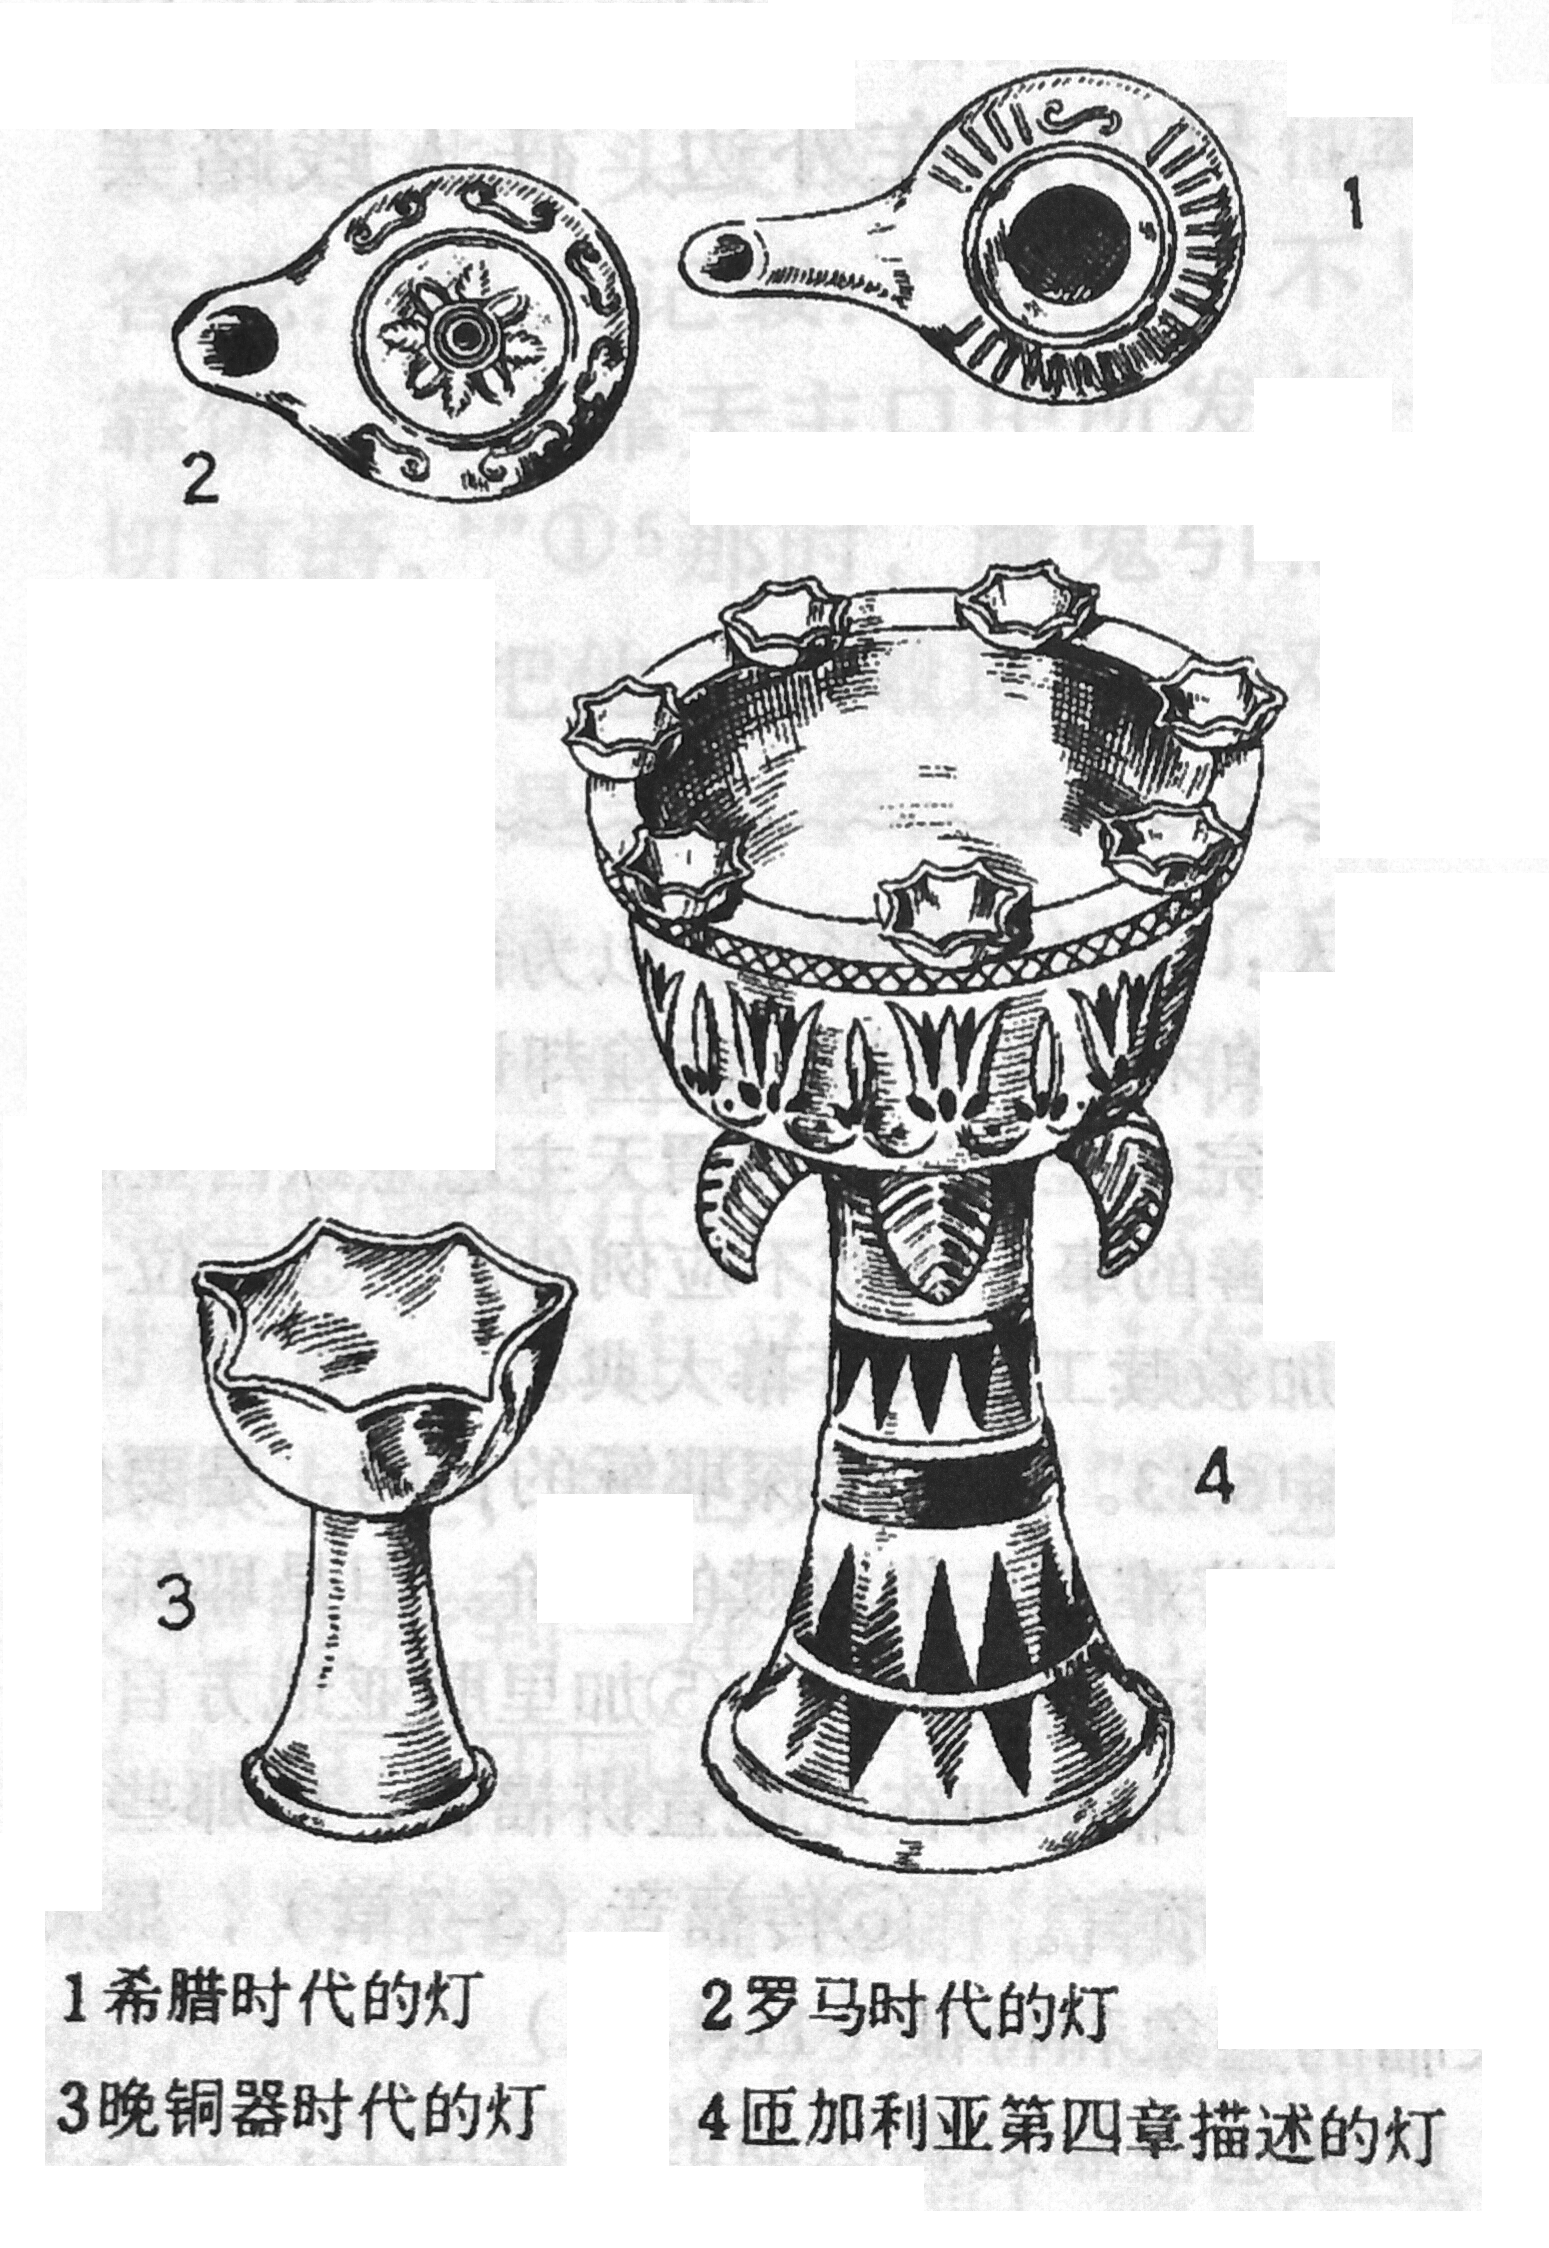
\includegraphics[width=72mm]{images/1514.png}
\end{center}


\subsubsection{新法律成全旧法律}
$^{17}$“你们不要以为我来是废除法律或先知;\textcircled{3}\NoLabelFootnote{5 \textcircled{3}法律与先知即指全部《旧约》。}我来不是为废除,而是为成全。$^{18}$我实在告诉你们:即使天地过去了,一撇或一画也决不会从法律上过去,必待一切完成。$^{19}$所以,谁若废除这些诫命中最小的一条,也这样教训人,在天国里,他将称为最小的;但谁若实行,也这样教训人,这人在天国里将称为大的。$^{20}$我告诉你们:除非你们的义德超过经师和\UL[法利塞]人的义德,你们决进不了天国。\textcircled{4}\NoLabelFootnote{5 \textcircled{4}基督徒的义德,是在于受法律的内外约束,而不是如\UL[法利塞]人所说,只在于法律的外在行为。}

$^{21}$你们一向听过给古人说:“不可杀人!”谁若杀了人,应受裁判。$^{22}$我却对你们说:凡向自己弟兄发怒的,就要受裁判;谁若向自己的弟兄说“傻子”,就要受议会的裁判;谁若说“疯子”,就要受火狱的罚。\textcircled{5}\NoLabelFootnote{5 \textcircled{5}\UL[耶稣]不但禁止人杀人,且也禁止人怀着导引人起杀机的愤怒和辱骂。“疯子”按原文是指不恭敬天主,不守法律的人。“火狱”按原文是指靠近\UL[耶路撒冷]城南烧垃圾和尸体的\UL[革厄纳]山谷(《旧约》常称\UL[本希农])。此山谷作了地狱的象征。}$^{23}$所以,你若在祭坛前,要献你的礼物时,在那里想起你的弟兄有什么怨你的事,$^{24}$就把你的礼物留在那里,留在祭坛前,先去与你的弟兄和好,然后再来献你的礼物。$^{25}$当你和你的对头还在路上,赶快与他和解,免得对头把你交与判官,判官交给差役,把你投在狱里。$^{26}$我实在告诉你:非到你还了最后的一文,决不能从那里出来。

$^{27}$你们一向听说过:“不可奸淫!”$^{28}$我却对你们说:凡注视妇女,有意贪恋她的,他已在心里奸淫了她。$^{29}$若是你的右眼使你跌倒,剜出它来,从你身上扔掉,因为丧失你一个肢体,比你全身投入地狱里,为你更好;$^{30}$若你的右手使你跌倒,砍下它来,从你身上扔掉,因为丧失你一个肢体,比你全身投入地狱里,为你更好。

$^{31}$又说过:“谁若休妻,就该给她休书。”$^{32}$我却给你们说:除了姘居外,凡休自己的妻子的,便是叫她受奸污;并且谁若娶被休的妇人,就是犯奸淫。\textcircled{6}\NoLabelFootnote{5 \textcircled{6}详见19:3-10并注。}

$^{33}$你们又一向听过对古人说:“不可发虚誓!要向上主偿还你的誓愿!”$^{34}$我却对你们说:你们总不可发誓:不可指天,因为天是天主的宝座;$^{35}$不可指地,因为地是他的脚凳;不可指\UL[耶路撒冷],因为她是大王的城市;$^{36}$也不可指你的头发誓,因为你不能使一根头发变白或变黑。$^{37}$你们的话该当是:是就说是,非就说非;其他多余的,便是出于邪恶。\textcircled{7}\NoLabelFootnote{5 \textcircled{7}17-37节,教训人守一切法律。预防犯罪,应由约束内心作起,\UL[法利塞]人即忽略了这一点。}

$^{38}$你们一向听说过:“以眼还眼,以牙还牙。”$^{39}$我却对你们说:不要抵抗恶人;而且,若有人掌击你的右颊,你把另一面也转给他。$^{40}$那愿与你争讼,拿你的内衣的,你连外衣也让给他。$^{41}$若有人强迫你走一千步,你就同他走两千步。$^{42}$求你的,就给他;愿向你借贷的,你不要拒绝。

$^{43}$你们一向听说过:“你应爱你的近人,恨你的仇人!”$^{44}$我却对你们说:你们当爱你们的仇人,当为迫害你们的人祈祷,$^{45}$好使你们成为你们在天之父的子女,因为他使太阳上升,光照恶人,也光照善人;降雨给义人,也给不义的人。$^{46}$你们若只爱那爱你们的人,你们还有什么赏报呢?税吏不是也这样作吗?$^{47}$你们若只问候你们的弟兄,你们作了什么特别的呢?外邦人不是也这样作吗?$^{48}$所以你们应当是成全的,如同你们的天父是成全的一样。”\textcircled{8}\NoLabelFootnote{5 \textcircled{8}基督徒的成全之德是爱,这爱尤其表现于爱仇人。爱仇非出于怯懦,而是效法天父恩待善人也恩待恶人的美德。}


\subsection{第六章 施舍祈祷和禁食的精神}
$^{1}$“你们应当心,不要在人前行你们的仁义,\textcircled{1}\NoLabelFootnote{6 \textcircled{1}“仁义”是泛指施舍、祈祷、禁食等善工。}为叫他们看见;若是这样,你们在天父之前,就没有赏报了。$^{2}$所以,当你施舍时,不可在你前面吹号,如同假善人在会堂及街市上所行的一样,为受人们的称赞;我实在告诉你们,他们已获得了他们他们的赏报。$^{3}$当你施舍时,不要叫你左手知道你右手所行的,$^{4}$好使你的施舍隐而不露,你父在暗中看见,必要报答你。$^{5}$当你祈祷时,不要如同假善人一样,爱在会堂及十字街头立着祈祷,为显示给人;我实在告诉你们,他们已获得了他们的赏报。\textcircled{2}\NoLabelFootnote{6 \textcircled{2}\UL[耶稣]不是指摘公众敬礼,而是指摘不由衷,只图炫耀于人的敬礼。}$^{6}$至于你,当你祈祷时,要进入你的内室,关上门,向你在暗中之父祈祷;你的父在暗中看见,必要报答你。

$^{7}$你们祈祷时,不要唠唠叨叨,如同外邦人一样,因为他们以为只要多言,便可获得垂允。$^{8}$你们不要跟他们一样,因为你们的父,在你们求他以前,已知道你们需要什么。$^{9}$所以,你们应当这样祈祷:

我们在天的父!愿你的名被尊为圣,

$^{10}$愿你的国来临,愿你的旨意承行于地,如在天上一样!

$^{11}$我们的日用粮,求你今天赐给我们;

$^{12}$宽免我们的罪债,犹如我们也宽免得罪我们的人;

$^{13}$不要让我们陷入诱惑,但救我们免于凶恶。\textcircled{3}\NoLabelFootnote{6 \textcircled{3}“天主经”是\UL[耶稣]亲自所传授的最完善的祈祷方式:前段求天主获得光荣,天国成立在世界上,世人承行主旨;后段求个人的日用急需,罪之赦,不为诱惑所陷害。参阅\uwave{路}11:2-4所载“天主经”。}

$^{14}$因为你们若宽免别人的过犯,你们的天父也必宽免你们的;$^{15}$但你们若不宽免别人的,你们的父也必不宽免你们的过犯。$^{16}$几时你们禁食,不要如同假善人一样,面带愁容;因为他们苦丧着脸,是为叫人看出他们禁食来。我实在告诉你们,他们已获得了他们的赏报。$^{17}$至于你,当你禁食时,要用油抹你的头,洗你的脸,$^{18}$不要叫人看出你禁食来,但叫你那在暗中之父看见;你的父在暗中看见,必要报答你。”


\subsubsection{归向天主的纯洁之心}
$^{19}$“你们不要在地上为自己积蓄财宝,因为在地上有虫蛀,有锈蚀,在地上也有贼挖洞偷窃;$^{20}$但该在天上为自己积蓄财宝,因为那里没有虫蛀,没有锈蚀,那里也没有贼挖洞偷窃。$^{21}$因为你的财宝在哪里,你的心也必在哪里。$^{22}$眼睛就是身体的灯。所以,你的眼睛若是康健,你的全身就都光明。$^{23}$但是,如果你的眼睛有了病,你的全身就都黑暗。那么,你身上的光明如果成了黑暗,那该是多么黑暗!”\textcircled{4}\NoLabelFootnote{6 \textcircled{4}以眼喻人心:如人心不为物欲所迷,只想望天上之事,人的生活自然合乎法度;不然,必定是非不分(\uwave{路}11:34-36)。}


\subsubsection{惟独事奉主依恃主的照顾}
$^{24}$“没有人能事奉两个主人:他或是要恨这一个而爱那一个,或是依附这一个而轻忽那一个。你们不能事奉天主而又事奉钱财。

$^{25}$为此,我告诉你们:不要为你们的生命忧虑吃什么,或喝什么;也不要为你们的身体忧虑穿什么。难道生命不是贵于食物,身体不是贵于衣服吗?$^{26}$你们仰观天空的飞鸟,它们不播种,也不收获,也不在粮仓里屯积,你们的天父还是养活它们;你们不比它们更贵重吗?$^{27}$你们中谁能运用思虑,使自己的寿数增加一肘呢?\textcircled{5}\NoLabelFootnote{6 \textcircled{5}“一肘”即言一会儿工夫。此句亦可译作:“使自己的身量增加一肘呢”。}$^{28}$关于衣服,你们又忧虑什么?你们观察一下田间的百合花怎样生长:它们既不劳作,也不纺织;$^{29}$可是我告诉你们:连\UL[撒罗满]在他极盛的荣华时代所披戴的,也不如这些花中的一朵。$^{30}$田地里的野草今天还在,明天就投在炉中,天主尚且这样装饰,信德薄弱的人那,何况你们呢?$^{31}$所以,你们不要忧虑说:我们吃什么,喝什么,穿什么?$^{32}$因为这一切都是外邦人所寻求的;你们的天父原晓得你们需要这一切。$^{33}$你们先该寻求天主的国和它的义德,这一切自会加给你们。$^{34}$所以你们不要为明天忧虑,因为明天有明天的忧虑:一天的苦足够一天受的了。”


\subsection{第七章 各种劝谕}
$^{1}$“你们不要判断人,免得你们受判断,$^{2}$因为你们用什么判断来判断,你们也要受什么判断;你们用什么尺度量给人,也要用什么尺度量给你们。$^{3}$为什么你只看见你兄弟眼中的木屑,而对自己眼中的大梁竟不理会呢?$^{4}$或者,你怎能对你的兄弟说:让我把你眼中的木屑取出来,而你眼中却有一根大梁呢?$^{5}$假善人哪!先从你眼中取出大梁,然后你才看得清楚,取出你兄弟眼中的木屑。

$^{6}$你们不要把圣物给狗,也不要把你们的珠宝投在猪前,怕它们用脚践踏了珠宝,而又转过来咬伤你们。\textcircled{1}\NoLabelFootnote{7 \textcircled{1} 圣物珠宝,指神圣的奥理,狗和猪,指心怀恶意的人。}

$^{7}$你们求,必要给你们;你们找,必要找着;你们敲,必要给你们开,$^{8}$因为凡是求的,就必得到;找的,就必找到;敲的,就必给他开。$^{9}$或者,你们中间有哪个人,儿子向他求饼,反而给他石头呢?$^{10}$或者求鱼,反而给他蛇呢?$^{11}$你们纵然不善,尚且知道把好的东西给你们的儿女,何况你们在天之父,岂不更将好的赐与求他的人?

$^{12}$所以,凡你们愿意人给你们做的,你们也要照样给人做:法律和先知即在于此。”\textcircled{2}\NoLabelFootnote{7 \textcircled{2} 旧约的总纲也不外是爱人如己。}


\subsubsection{辨别真假好坏的训言}
$^{13}$“你们要从窄门进去,因为宽门和大路导入丧亡;但有许多的人从那里进去。$^{14}$那导人生命的门是多么窄,路是多么狭!找到它的人的确不多。\textcircled{3}\NoLabelFootnote{7 \textcircled{3} 窄门狭路指守诫命,背十字架的生活。}

$^{15}$你们要提防假先知!他们来到你们跟前,外披羊毛,内里却是凶残的豺狼。$^{16}$你们可凭他们的果实辨别他们:荆棘上岂能收到葡萄?或者蒺藜上岂能收到无花果?$^{17}$这样,凡是好树都结好果子,而坏树都结坏果子;$^{18}$好树不能结坏果子,坏树也不能结好果子。$^{19}$凡不结好果子的树,必要砍倒,投入火中。$^{20}$所以,你们可凭他们的果实辨别他们。

$^{21}$不是凡向我们“主啊!主啊!”的人,就能进天国;而是那承行我在天之父旨意的人,才能进天国。$^{22}$到那一天有许多人要向我说:主啊!主啊!我们不是因你的名字说过预言,因你的名字驱过魔鬼,因你的名字行过许多奇迹吗?$^{23}$那时,我必要向他们声明说:我从来不认识你们,你们这些作恶的人,离开我吧!”


\subsubsection{山中圣训的结论}
${24}$“所以,凡听了我这些话而实行的,就好像一个聪明人,把自己的房屋建在磐石上:${25}$雨淋,水冲,风吹,袭击那座房屋,它并不坍塌,因为基础是建在磐石上。${26}$凡听了我这些话而不实行的,就好像一个愚昧人,把自己的房屋建在沙土上:${27}$雨淋,水冲,风吹,袭击那座房屋,它就坍塌了,且坍塌的很惨。”

${28}$\UL{耶稣}讲完了这些话,群众都惊奇他的教训,${29}$因为他教训他们,正像有权威的人,不像他们他们的经师。


\section{建立天国的准备 耶稣行的奇迹}

\end{document}